\chapter{Trocas gasosas respiratórias}\label{ch:b1:gas-exchange}

Um litro de ar contém trinta vezes mais oxigênio do que um litro de
água, pesa oitocentas vezes menos e deixa o oxigênio difundir-se
através dele dez mil vezes mais depressa. Uma truta precisa fazer
passar cento e cinquenta gramas de água pelas \omterm{def:b1:gas-exchange:gill}{brânquias} por cada
miligrama de oxigênio que retira, e extrai quatro quintos do que a
água transporta; um ser humano move alguns gramas de ar por miligrama
e desperdiça três quartos deles. Os dois \omterm{def:b1:mammal-organization:organ}{órgãos} são respostas à mesma
equação --- o fluxo de um gás através de uma superfície --- em dois
meios. Este capítulo enuncia a física, deduz o que uma \omterm{prop:b1:organism-environment:surfaces}{superfície de
troca} tem de ser, descreve \omterm{def:b1:gas-exchange:gill}{brânquias}, \omterm{def:b1:gas-exchange:lung}{pulmões} e traqueias, segue o
oxigênio e o dióxido de carbono através do sangue e examina como a
ventilação é controlada e o que muda em altitude e debaixo de água.

\section{A física de um gás em dois meios}

\begin{definition}[Pressão parcial, solubilidade]\label{def:b1:gas-exchange:partial}
\index{pressão parcial}
Numa mistura de gases, cada gás exerce uma \emph{pressão parcial}
proporcional à sua fração: no ar a \qty{101}{kPa}, o oxigênio
(\qty{20.9}{\%}) tem $P_{\mathrm{O_2}} = \qty{21.2}{kPa}$, o dióxido
de carbono (\qty{0.04}{\%}) \qty{0.04}{kPa}. Um gás dissolve-se num
líquido em proporção à sua pressão parcial (lei de Henry): a água em
equilíbrio com o ar a \qty{15}{\celsius} contém \qty{0.32}{mmol/L} de
oxigênio (\qty{10}{mg/L}, \qty{7}{mL/L} de gás), contra
\qty{8.7}{mmol/L} (\qty{210}{mL/L}) no próprio ar. A pressão parcial
--- a mesma na água e no ar em equilíbrio --- é o que impulsiona a
difusão entre os meios; o conteúdo é o que um respirador pode extrair.
O dióxido de carbono é vinte e cinco vezes mais solúvel do que o
oxigênio, e por isso nunca é o gás mais difícil de trocar.
\end{definition}

\begin{theorem}[Lei de Fick para uma superfície de troca]\label{thm:b1:gas-exchange:fick}
\index{lei de Fick}
A velocidade com que um gás atravessa uma membrana de área $A$ e
espessura $x$ que separa dois meios às pressões parciais $P_1$ e $P_2$ é
\[
\dot V = K\,\frac{A}{x}\,(P_1 - P_2),
\]
onde $K$, a constante de difusão (de Krogh) da membrana, combina a
difusividade e a solubilidade do gás no \omterm{def:b1:body-plans-tissues:tissue}{tecido}. O fluxo é aumentado
por uma área maior, uma barreira mais fina e uma diferença de \omterm{def:b1:gas-exchange:partial}{pressão
parcial} maior; por nada mais.
\end{theorem}
\begin{proof}
A primeira \omterm{thm:b1:membranes-transport:fick}{lei de Fick} aplicada ao gás dissolvido na membrana
(\cref{ch:b1:membranes-transport}) dá um fluxo por unidade de área
proporcional ao gradiente de concentração; pela lei de Henry, a
concentração em cada face é proporcional à \omterm{def:b1:gas-exchange:partial}{pressão parcial} do meio
que lhe corresponde, de modo que o gradiente é $(P_1 - P_2)/x$ vezes
a solubilidade, e a constante absorve solubilidade e difusividade.
\end{proof}

\begin{omfigure}
\begin{tikzpicture}
\begin{axis}[
  ybar, bar width=16pt,
  width=0.72\linewidth, height=5.6cm,
  axis x line=bottom, axis y line=left,
  ymode=log, log origin=infty, ymin=0.1, ymax=3000,
  ylabel={oxigênio por litro de meio (\unit{mL})},
  ylabel style={font=\small},
  symbolic x coords={air, water at 5 C, water at 15 C, water at 30 C, sea water at 15 C},
  xticklabels={ar, água a 5 C, água a 15 C, água a 30 C, água do mar a 15 C},
  xtick=data, x tick label style={font=\small, rotate=20, anchor=north east},
  enlarge x limits=0.15,
  nodes near coords, nodes near coords style={font=\scriptsize, anchor=south},
  point meta=rawy,
]
\addplot[fill=omDef!45, draw=omDef] coordinates {(air,210) (water at 5 C,9.0) (water at 15 C,7.1) (water at 30 C,5.3) (sea water at 15 C,5.8)};
\end{axis}
\end{tikzpicture}

{\small Conteúdo de oxigênio do ar e da água em equilíbrio com ele. A
água contém trinta vezes menos, e menos ainda quando está quente ou
salgada: um peixe numa lagoa de verão vive no limite do suprimento.}
\end{omfigure}

\begin{proposition}[O que uma superfície de troca tem de ser]\label{prop:b1:gas-exchange:requirements}
\index{superfície de troca}
Um \omterm{def:b1:organism-environment:organism}{organismo} com mais de um milímetro não pode ser abastecido por
difusão através da sua superfície externa
(\cref{ch:b1:organism-environment}). Precisa de uma \emph{superfície
respiratória} que seja ampla (para aumentar $A$), fina (para diminuir
$x$), úmida (os gases só atravessam membranas em solução),
\emph{ventilada} --- o meio externo renovado, para que $P_1$ se
mantenha alto --- e \emph{perfundida} --- o sangue por trás dela
renovado, para que $P_2$ se mantenha baixo; e de uma circulação que
leve o gás da superfície aos \omterm{def:b1:body-plans-tissues:tissue}{tecidos}. \omterm{def:b1:gas-exchange:gill}{Brânquias}, \omterm{def:b1:gas-exchange:lung}{pulmões} e traqueias
são três maneiras de dobrar tal superfície dentro de um corpo e de
fazer os dois fluidos passarem por ela.
\end{proposition}

\section{Brânquias e a contracorrente}

\begin{definition}[Brânquia]\label{def:b1:gas-exchange:gill}
\index{brânquia}
Uma \emph{brânquia} é uma evaginação da superfície do corpo para
dentro da água, dobrada em filamentos e \emph{lamelas} de alguns
micrômetros de espessura, através das quais o sangue corre em
capilares. As brânquias de um peixe pendem de quatro arcos ósseos de
cada lado; a água aspirada pela boca e expulsa por baixo dos opérculos
por um sistema de duas bombas corre entre as lamelas num sentido, e o
sangue nas lamelas corre no sentido oposto: uma
\emph{contracorrente}\index{troca em contracorrente}.
Uma truta de um quilograma tem cerca de \qty{2000}{cm^2} de superfície
lamelar, com \qty{2}{\micro m} de espessura.
\end{definition}

\begin{omfigure}
\begin{tikzpicture}
  \node[anchor=south west, inner sep=0] (img) at (0,0)
    {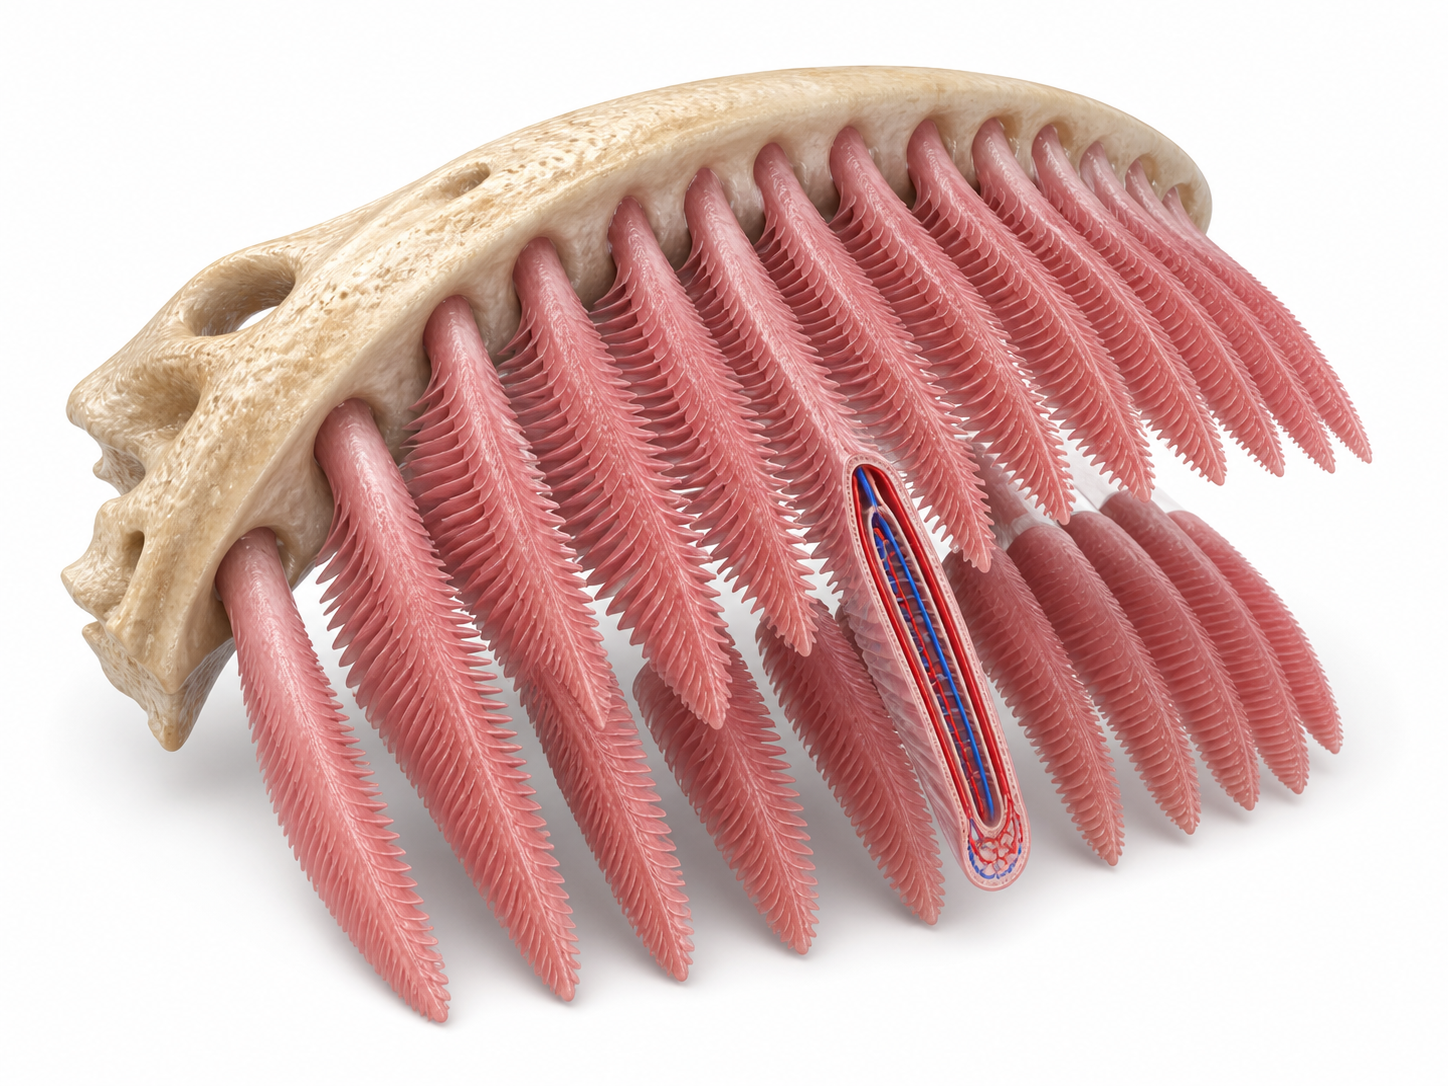
\includegraphics[width=0.52\linewidth]{images/book3/ai/fig-gill-lamellae.png}};
  \begin{scope}[x={(img.south east)}, y={(img.north west)},
      every node/.style={font=\small}]
    \draw[omDef, thick] (0.20,0.50) -- (-0.03,0.60) node[left] {arco branquial};
    \draw[omDef, thick] (0.55,0.70) -- (0.55,1.08) node[above] {filamentos};
    \draw[omDef, thick] (0.75,0.40) -- (1.03,0.30) node[right, align=left] {lamelas: a superfície\\ de troca, \qty{2}{\micro m} de espessura};
    \draw[omDef, thick] (0.45,0.20) -- (0.45,-0.08) node[below] {vasos sanguíneos ao longo do filamento};
  \end{scope}
\end{tikzpicture}

{\small Um arco branquial com seus filamentos e suas lamelas. A água
corre entre as lamelas; o sangue corre através delas em sentido oposto.}
\end{omfigure}

\begin{theorem}[Troca em contracorrente]\label{thm:b1:gas-exchange:countercurrent}
Quando a água e o sangue correm em sentidos opostos ao longo de uma
\omterm{prop:b1:organism-environment:surfaces}{superfície de troca}, o sangue que sai da \omterm{def:b1:gas-exchange:gill}{brânquia} pode aproximar-se da
\omterm{def:b1:gas-exchange:partial}{pressão parcial} da água que \emph{entra} nela, e a água pode ser
despojada da maior parte do seu oxigênio: extrações de \qty{80}{\%} ou
mais. Quando correm no mesmo sentido (cocorrente), os dois fluidos
convergem para um valor intermediário comum e a extração não pode
ultrapassar \qty{50}{\%}.
\end{theorem}
\begin{proof}
Ao longo de um trocador em cocorrente, a diferença $P_{\text{água}} -
P_{\text{sangue}}$ cai do seu valor de entrada até zero à medida que
os dois se aproximam da mesma pressão; uma vez iguais, nenhum gás se
move mais, e para fluxos iguais o ponto de encontro fica a meio
caminho. Em fluxo em \omterm{def:b1:gas-exchange:gill}{contracorrente}, o sangue, ao avançar para a sua
saída, encontra água cada vez mais fresca, de modo que uma diferença
positiva se mantém ao longo de todo o comprimento; o sangue na sua
saída enfrenta a água que entra a \qty{21}{kPa}, e a água na sua saída
enfrenta o sangue venoso que entra a alguns quilopascais. O limite é
imposto pela superfície, não por um equilíbrio.
\end{proof}

\begin{omfigure}
\begin{tikzpicture}[font=\footnotesize, >=Stealth, line cap=round]
  % co-current
  \begin{scope}
    \node[anchor=south, font=\small] at (2.6,1.65) {cocorrente: os dois fluxos no mesmo sentido};
    \draw[->, very thick, omDef] (0,1.2) -- (5.2,1.2) node[right] {saída de água: \qty{12}{kPa}};
    \draw[->, very thick, omThm] (0,0.4) -- (5.2,0.4) node[right] {saída de sangue: \qty{12}{kPa}};
    \node[anchor=east, omDef] at (-0.1,1.2) {entrada de água: \qty{21}{kPa}};
    \node[anchor=east, omThm] at (-0.1,0.4) {entrada de sangue: \qty{3}{kPa}};
    \foreach \x/\d in {0.6/18, 1.6/12, 2.6/7, 3.6/3, 4.6/0.5} { \draw[->, gray] (\x,1.05) -- (\x,0.55) node[midway, right, font=\scriptsize, gray] {\d}; }
    \node[anchor=north, align=center] at (2.6,0.1) {a diferença (cinza, kPa) diminui até zero:\\ a extração para em \qty{43}{\%}};
  \end{scope}
  \begin{scope}[yshift=-3.6cm]
    \node[anchor=south, font=\small] at (2.6,1.65) {contracorrente: fluxos opostos};
    \draw[->, very thick, omDef] (0,1.2) -- (5.2,1.2) node[right] {saída de água: \qty{4}{kPa}};
    \draw[<-, very thick, omThm] (0,0.4) -- (5.2,0.4) node[right] {entrada de sangue: \qty{3}{kPa}};
    \node[anchor=east, omDef] at (-0.1,1.2) {entrada de água: \qty{21}{kPa}};
    \node[anchor=east, omThm] at (-0.1,0.4) {saída de sangue: \qty{18}{kPa}};
    \foreach \x/\d in {0.6/3, 1.6/3, 2.6/3, 3.6/3, 4.6/2} { \draw[->, gray] (\x,1.05) -- (\x,0.55) node[midway, right, font=\scriptsize, gray] {\d}; }
    \node[anchor=north, align=center] at (2.6,0.1) {a diferença mantém-se positiva ao longo de todo o percurso:\\ a extração chega a \qty{80}{\%} e o sangue sai perto do valor de entrada da água};
  \end{scope}
\end{tikzpicture}

{\small Troca em cocorrente e em \omterm{def:b1:gas-exchange:gill}{contracorrente} com a mesma superfície
e os mesmos fluxos. Opor os fluxos mantém um gradiente ao longo de
todo o percurso e permite que o sangue se aproxime da pressão de
oxigênio da água fresca.}
\end{omfigure}

\begin{omfigure}
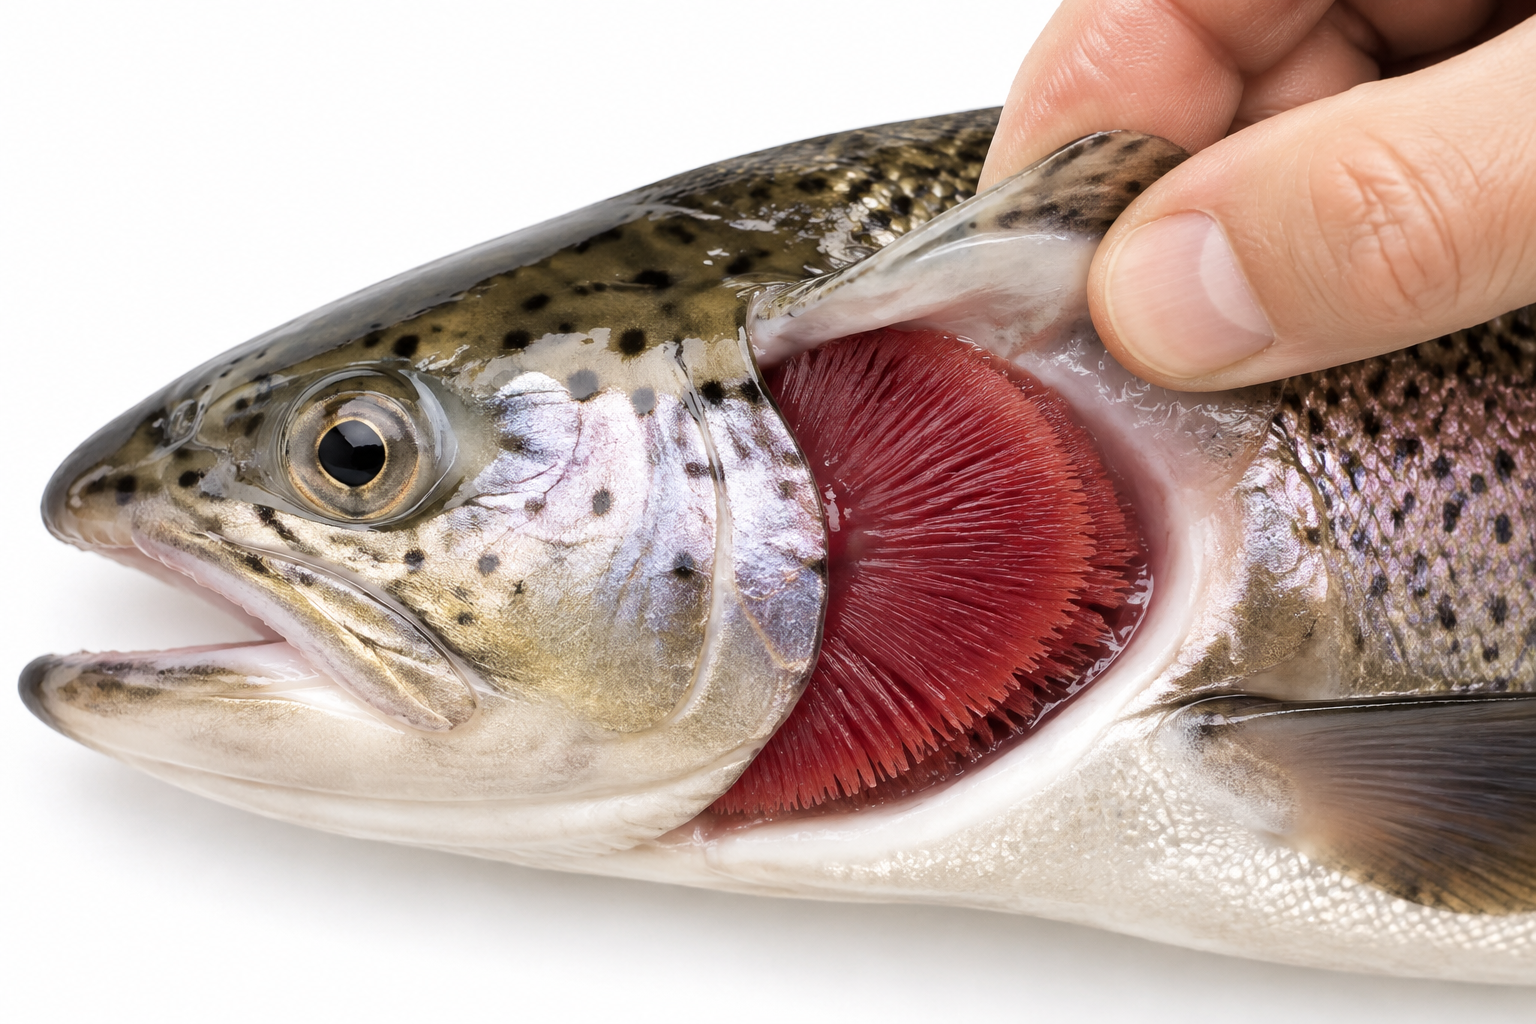
\includegraphics[width=0.5\linewidth]{images/book3/ai/b3-21-trout-gills.png}

{\small As \omterm{def:b1:gas-exchange:gill}{brânquias} de uma truta sob o opérculo levantado: vermelhas
de sangue, porque as lamelas têm duas \omterm{def:b1:cell-unit-of-life:cell}{células} de espessura e o sangue
fica a um micrômetro da água.}
\end{omfigure}

\begin{example}[O preço da água]\label{ex:b1:gas-exchange:priceofwater}
Uma truta em repouso de \qty{1}{kg} consome cerca de \qty{50}{mL} de
oxigênio por hora. A partir de água com \qty{7}{mL/L}, com
\qty{80}{\%} de extração, precisa bombear \qty{9}{L} de água por hora
pelas \omterm{def:b1:gas-exchange:gill}{brânquias} --- nove quilogramas de um meio cinquenta vezes mais
viscoso do que o ar, por \omterm{def:b1:membranes-transport:transporters}{canais} com uma fração de milímetro de
largura. Um décimo do seu metabolismo vai para a respiração; um ser
humano em repouso gasta um cinquentavo. Aqueça a lagoa até
\qty{30}{\celsius} e o mesmo peixe, precisando de mais oxigênio de uma
água que contém menos, terá de bombear três vezes mais.
\end{example}

\section{Respirar ar: pulmões e traqueias}

\begin{definition}[O pulmão dos mamíferos]\label{def:b1:gas-exchange:lung}
\index{pulmão}\index{alvéolo}
Um \emph{pulmão} é uma invaginação da superfície do corpo para dentro
de uma câmara interna úmida, o que mantém a superfície molhada em ar
seco. O pulmão dos mamíferos é uma árvore de vias aéreas que termina
em cerca de trezentos milhões de \emph{alvéolos}, sacos de
\qty{0.2}{mm} de diâmetro cujas paredes --- uma \omterm{def:b1:cell-unit-of-life:cell}{célula} epitelial e um
endotélio capilar, \qty{0.5}{\micro m} ao todo --- somam
\qty{100}{m^2} num ser humano, envolvidos por uma rede capilar por
onde passa todo o débito cardíaco. É ventilado por \emph{volume
corrente}: o \omterm{def:b1:mammal-organization:bodyplan}{diafragma} e os músculos intercostais alargam o tórax e o
ar entra; relaxam e o ar sai pelo mesmo caminho. Uma respiração move
\qty{500}{mL}, dos quais \qty{150}{mL} apenas enchem as vias aéreas
(\emph{espaço morto}) e nunca chegam a um alvéolo; o gás alveolar,
renovado em um sétimo a cada respiração, mantém-se a $P_{\mathrm{O_2}} =
\qty{13.3}{kPa}$ e $P_{\mathrm{CO_2}} = \qty{5.3}{kPa}$ --- as
pressões com que o sangue se equilibra.
\end{definition}

\begin{omfigure}
\begin{tikzpicture}
  \node[anchor=south west, inner sep=0] (img) at (0,0)
    {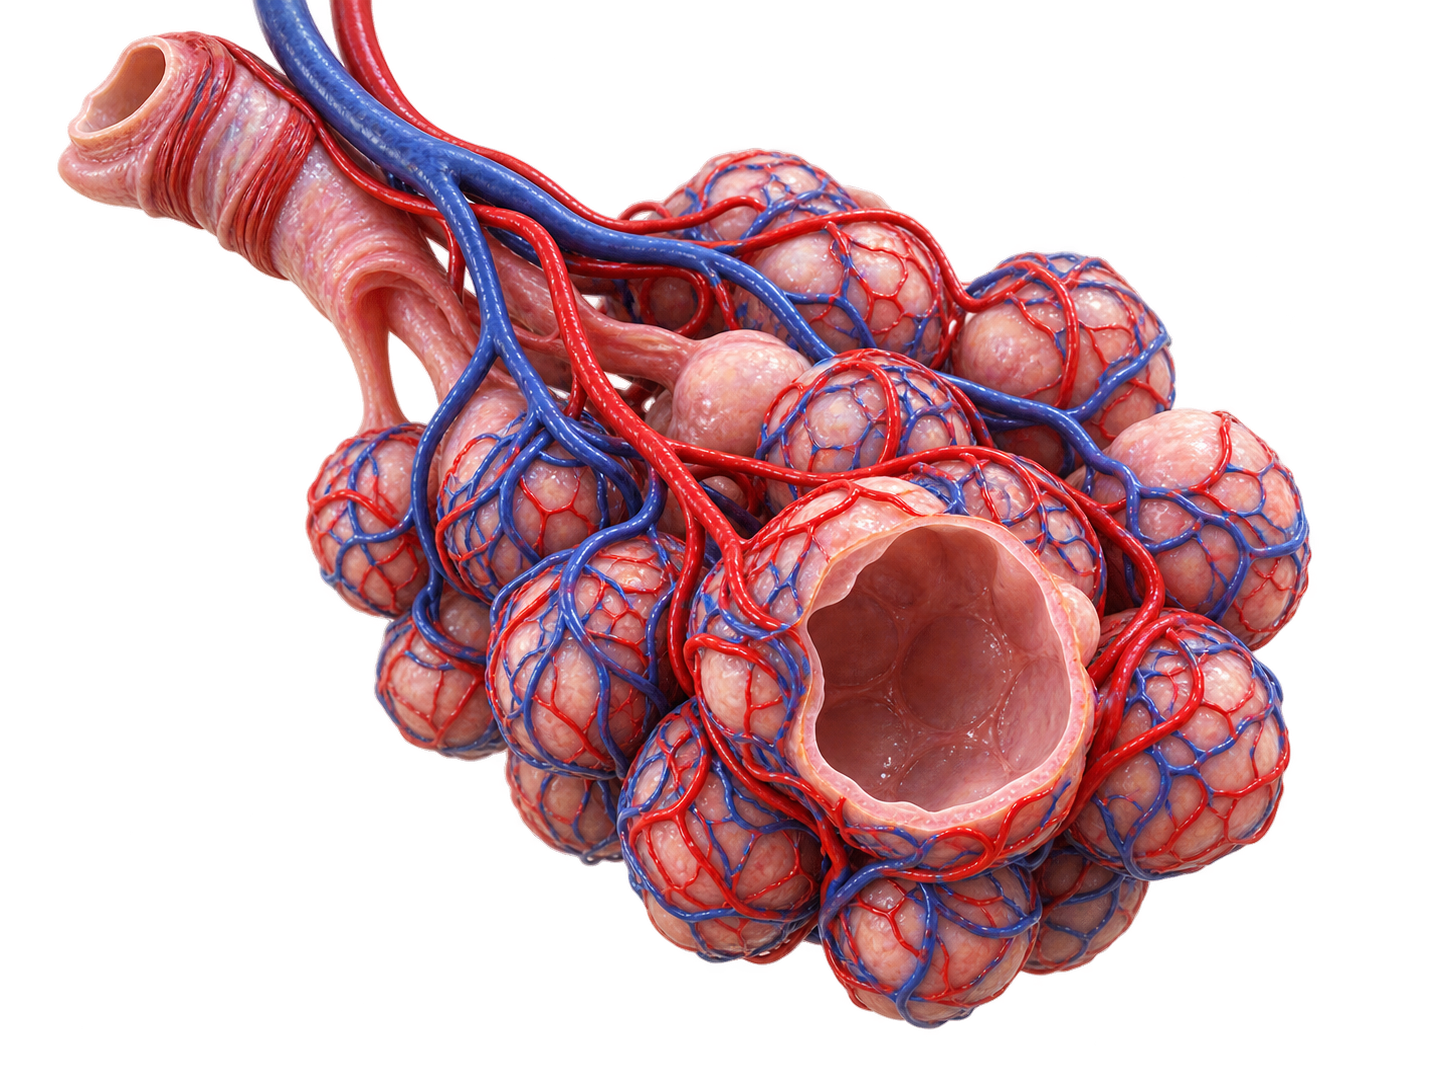
\includegraphics[width=0.5\linewidth]{images/book3/ai/fig-alveoli.png}};
  \begin{scope}[x={(img.south east)}, y={(img.north west)},
      every node/.style={font=\small}]
    \draw[omDef, thick] (0.50,0.85) -- (0.50,1.08) node[above] {via aérea terminal};
    \draw[omDef, thick] (0.30,0.45) -- (-0.03,0.40) node[left, align=right] {alvéolo aberto:\\ ar no interior};
    \draw[omDef, thick] (0.75,0.55) -- (1.03,0.62) node[right, align=left] {rede capilar\\ na parede};
    \draw[omDef, thick] (0.60,0.15) -- (0.60,-0.08) node[below] {parede: \qty{0.5}{\micro m} entre o ar e o sangue};
  \end{scope}
\end{tikzpicture}

{\small \omterm{def:b1:gas-exchange:lung}{Alvéolos} no fim de uma via aérea, envolvidos por capilares.
Todo o débito cardíaco se espalha por uma centena de metros quadrados
desta parede, uma fração de segundo de cada vez.}
\end{omfigure}

\begin{proposition}[Três projetos para o ar]\label{prop:b1:gas-exchange:designs}
\index{traqueias}
Os \emph{mamíferos} ventilam por volume corrente: é simples, mas o ar
fresco mistura-se com o viciado, o oxigênio alveolar é dois terços do
atmosférico e a extração é de um quarto. As \emph{aves} fazem o ar
passar num único sentido por tubos finos (parabrônquios) entre dois
conjuntos de sacos aéreos que funcionam como foles, de modo que ar
fresco atravessa a \omterm{prop:b1:organism-environment:surfaces}{superfície de troca} tanto na inspiração como na
expiração, em corrente cruzada com o sangue: sua extração é maior, e
um ganso-indiano voa sobre o Himalaia onde um mamífero desmaiaria. Os
\emph{insetos} não têm sangue respiratório nenhum: o ar entra por
válvulas (\emph{espiráculos}) para \emph{traqueias}, tubos rijos
graças a espessamentos em espiral, que se ramificam até o micrômetro e
entregam oxigênio por difusão diretamente a cada \omterm{def:b1:cell-unit-of-life:cell}{célula}, com o auxílio
do bombeamento do abdome nos insetos grandes ou ativos. A difusão ao
longo de tubos limita o projeto a corpos pequenos --- o que é uma das
razões por que nenhum inseto é maior do que um camundongo.
\end{proposition}

\begin{omfigure}
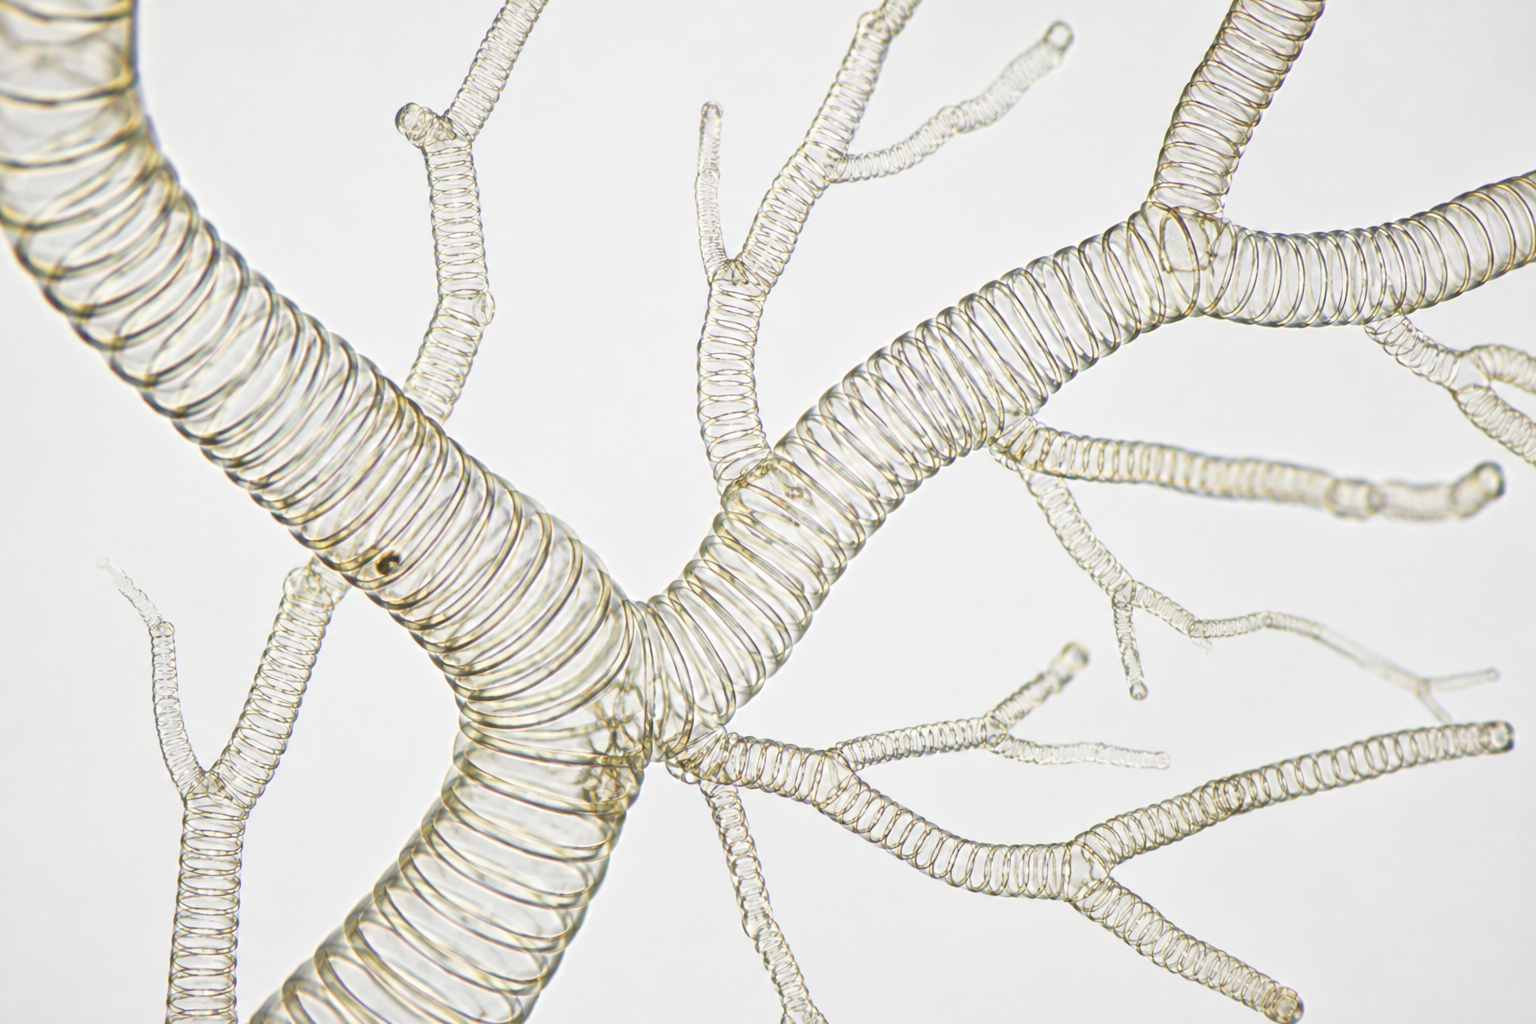
\includegraphics[width=0.5\linewidth]{images/book3/ai/b3-21-insect-tracheae.png}

{\small Traqueias de inseto: tubos cheios de ar mantidos abertos por
espessamentos em espiral, ramificando-se até as \omterm{def:b1:cell-unit-of-life:cell}{células}. Nenhum sangue
transporta o oxigênio; o ar vai até o fim.}
\end{omfigure}

\begin{method}[Ler um balanço de ventilação]\label{met:b1:gas-exchange:budget}
\begin{enumerate}
  \item Ventilação-minuto $=$ volume corrente $\times$ frequência
        respiratória; ventilação alveolar $=$ (volume corrente $-$
        espaço morto) $\times$ frequência respiratória. Só a segunda
        troca gás.
  \item Consumo de oxigênio $=$ ventilação alveolar $\times$ (fração
        inspirada $-$ fração alveolar); em repouso,
        $\qty{4.2}{L/min}\times(0.21 - 0.14) \approx \qty{0.3}{L/min}$.
  \item Extração $=$ consumo $/$ (ventilação $\times$ fração
        inspirada): um quarto num \omterm{def:b1:gas-exchange:lung}{pulmão} de ventilação corrente,
        quatro quintos numa \omterm{def:b1:gas-exchange:gill}{brânquia} em \omterm{def:b1:gas-exchange:gill}{contracorrente}.
  \item Do lado do sangue: consumo $=$ débito cardíaco $\times$
        (conteúdo arterial $-$ venoso); \qty{5}{L/min}$\times$
        \qty{50}{mL/L} em repouso, os mesmos \qty{250}{mL/min}. Os
        dois balanços têm de coincidir.
\end{enumerate}
\end{method}

\section{Os gases no sangue}

\begin{proposition}[Transporte de oxigênio e de dióxido de carbono]\label{prop:b1:gas-exchange:transport}
\index{anidrase carbônica}\index{efeito Bohr}\index{efeito Haldane}
O plasma dissolve apenas \qty{3}{mL} de oxigênio por litro à pressão
arterial; a hemoglobina (\cref{ch:b1:proteins}) transporta
\qty{200}{mL}, carregando-se no \omterm{def:b1:gas-exchange:lung}{pulmão} a \qty{13.3}{kPa} e
descarregando de um quinto a metade nos \omterm{def:b1:body-plans-tissues:tissue}{tecidos}. O dióxido de carbono
viaja de três maneiras: \qty{7}{\%} dissolvido, \qty{23}{\%} ligado
aos grupos amino da hemoglobina e \qty{70}{\%} como bicarbonato: na
hemácia, a \emph{\omterm{prop:b1:gas-exchange:transport}{anidrase carbônica}} converte $\mathrm{CO_2}$ e água
em ácido carbônico em milissegundos, o ácido se dissocia, o
bicarbonato sai da \omterm{def:b1:cell-unit-of-life:cell}{célula} em troca de cloreto (o \emph{desvio do
cloreto}) e o próton é captado pela hemoglobina. Os dois gases se
ajudam mutuamente: o ácido e o $\mathrm{CO_2}$ baixam a afinidade da
hemoglobina pelo oxigênio (\emph{\omterm{prop:b1:gas-exchange:transport}{efeito Bohr}}), de modo que o oxigênio
é liberado onde o $\mathrm{CO_2}$ é produzido; e a hemoglobina
desoxigenada liga melhor prótons e $\mathrm{CO_2}$ (\emph{\omterm{prop:b1:gas-exchange:transport}{efeito
Haldane}}), de modo que o $\mathrm{CO_2}$ é captado onde o oxigênio é
liberado, e cedido no \omterm{def:b1:gas-exchange:lung}{pulmão} à medida que o oxigênio se carrega.
\end{proposition}

\begin{omfigure}
\begin{tikzpicture}[font=\footnotesize, >=Stealth, line cap=round]
  % red cell
  \draw[very thick, omThm!80!black, fill=omThm!8, rounded corners=18pt] (0,0) rectangle (7.6,4.0);
  \node[anchor=north west, omThm!80!black, font=\small] at (0.15,3.95) {hemácia (num capilar de um tecido)};
  % CO2 in from tissue
  \draw[->, very thick, omDef] (-1.6,2.6) -- (0,2.6) node[pos=0, left, align=right] {$\mathrm{CO_2}$ vindo\\ do tecido};
  \node[draw, thick, fill=white, rounded corners=3pt, inner sep=2pt] (ca) at (2.0,2.6) {$\mathrm{CO_2} + \mathrm{H_2O} \to \mathrm{H_2CO_3}$};
  \node[anchor=south, font=\scriptsize, omProp!80!black] at (2.0,2.95) {anidrase carbônica};
  \node[draw, thick, fill=white, rounded corners=3pt, inner sep=2pt] (dis) at (5.2,2.6) {$\mathrm{H^+} + \mathrm{HCO_3^-}$};
  \draw[->, thick] (ca) -- (dis);
  % bicarbonate out, chloride in
  \draw[->, very thick, omDef] (6.2,2.4) -- (6.2,0.9) -- (8.4,0.9) node[right, align=left] {$\mathrm{HCO_3^-}$ para o plasma\\ (\qty{70}{\%} do $\mathrm{CO_2}$)};
  \draw[<-, very thick, gray] (6.9,1.85) -- (8.4,1.85) node[right, gray] {$\mathrm{Cl^-}$ em troca};
  % proton to Hb, O2 release
  \node[draw, thick, fill=omThm!25, rounded corners=3pt, inner sep=2pt] (hb) at (4.0,1.0) {hemoglobina};
  \draw[->, thick] (4.7,2.35) -- (4.2,1.3) node[midway, right, font=\scriptsize] {$\mathrm{H^+}$ ligado};
  \draw[->, very thick, omExo!70!black] (hb.west) -- (0,1.0) -- (-1.6,1.0) node[left, align=right] {$\mathrm{O_2}$ liberado\\ (efeito Bohr)};
  \node[anchor=north, align=center, gray] at (3.8,-0.2) {no pulmão cada seta se inverte: o oxigênio se carrega, prótons e $\mathrm{CO_2}$ são liberados,\\ o bicarbonato volta a entrar na célula e o $\mathrm{CO_2}$ é exalado};
\end{tikzpicture}

{\small O dióxido de carbono numa hemácia. A \omterm{prop:b1:gas-exchange:transport}{anidrase carbônica} produz
ácido carbônico; o bicarbonato sai para o plasma e o próton é captado
pela hemoglobina, que libera oxigênio ao ligá-lo.}
\end{omfigure}

\begin{example}[Um litro de sangue através de um músculo em trabalho]\label{ex:b1:gas-exchange:litre}
O sangue arterial traz \qty{200}{mL} de oxigênio por litro e
\qty{480}{mL} de dióxido de carbono (na maior parte como bicarbonato).
Num músculo em repouso deixa \qty{50}{mL} de oxigênio e capta
\qty{40}{mL} de $\mathrm{CO_2}$; o pH venoso cai apenas \qty{0.04}{},
porque a hemoglobina absorveu os prótons. Num músculo em disparada, a
pH 7,2 e com $P_{\mathrm{O_2}}$ de \qty{2.7}{kPa}, o mesmo litro deixa
\qty{150}{mL} de oxigênio (\cref{ch:b1:proteins}) e leva também o
lactato.
\end{example}

\section{Controle, altitude e mergulho}

\begin{proposition}[A ventilação é controlada pelo dióxido de carbono]\label{prop:b1:gas-exchange:control}
\index{quimiorreceptor}
O ritmo da respiração é gerado no tronco encefálico e ajustado por
\emph{quimiorreceptores}: os centrais, banhados pelo líquido que
rodeia o encéfalo, respondem à variação de pH que o $\mathrm{CO_2}$
produz; os periféricos, nas artérias carótidas, respondem a uma queda
do oxigênio arterial abaixo de cerca de \qty{8}{kPa}. Na vida corrente
é o $\mathrm{CO_2}$ que manda: uma subida de \qty{1}{kPa} na
$P_{\mathrm{CO_2}}$ arterial praticamente duplica a ventilação,
enquanto o oxigênio tem de cair um terço antes que a ventilação
responda. Prender a respiração termina quando o $\mathrm{CO_2}$, e não
o oxigênio, atinge o limite; hiperventilar antes baixa o
$\mathrm{CO_2}$ e permite ao mergulhador ficar submerso até que o
oxigênio acabe --- inconsciente antes que a vontade de respirar volte.
\end{proposition}

\begin{omfigure}
\begin{tikzpicture}
\begin{axis}[
  width=0.86\linewidth, height=5.8cm,
  axis x line=bottom, axis y line=left,
  xmin=4, xmax=8.5, ymin=0, ymax=45,
  xlabel={$P_{\mathrm{CO_2}}$ arterial (\unit{kPa})}, ylabel={ventilação (\unit{L/min})},
  xlabel style={font=\small, at={(axis description cs:0.5,-0.13)}, anchor=north},
  ylabel style={font=\small},
  tick label style={font=\small}, xtick={4,5,6,7,8}, ytick={0,10,20,30,40},
  legend style={font=\small, at={(0.03,0.97)}, anchor=north west, draw=none},
  clip=false,
]
\addplot[very thick, omDef, domain=4.5:8.5, samples=20] {6 + 10*(x-5.3)};
\addlegendentry{oxigênio normal}
\addplot[very thick, omThm, domain=4.5:7.2, samples=20] {6 + 20*(x-5.3)};
\addlegendentry{oxigênio baixo (\qty{7}{kPa}): mais inclinada}
\draw[dashed, gray] (axis cs:5.3,0) -- (axis cs:5.3,6); \node[font=\scriptsize, anchor=west] at (axis cs:5.4,1.5) {valor de repouso};
\end{axis}
\end{tikzpicture}

{\small Ventilação em função do dióxido de carbono arterial. Cada
quilopascal acima do valor de repouso acrescenta cerca de
\qty{10}{L/min}; o oxigênio baixo torna a resposta mais inclinada mas,
sozinho, pouco faz enquanto não for grave.}
\end{omfigure}

\begin{example}[Altitude e profundidade]\label{ex:b1:gas-exchange:altitudediving}
A \qty{4000}{m} o ar contém \qty{12}{kPa} de oxigênio e os \omterm{def:b1:gas-exchange:lung}{alvéolos}
\qty{7}{}: os corpos carotídeos elevam a ventilação, o que expulsa
$\mathrm{CO_2}$ e torna o sangue alcalino --- um freio que os rins
soltam ao longo de dias excretando bicarbonato; as hemácias aumentam
o seu BPG em poucos dias e a medula óssea aumenta a hemoglobina em
poucas semanas (\cref{ch:b1:proteins}). Uma foca que mergulha por
vinte minutos faz o contrário: expira antes de mergulhar, reduz o
coração a um décimo, fecha o sangue a tudo menos ao encéfalo e ao
coração, e faz os músculos funcionarem com o oxigênio ligado à sua
própria mioglobina, dez vezes mais concentrada do que a nossa, e
depois com \omterm{def:b1:respiration-fermentation:fermentation}{fermentação}, tolerando um lactato que o corpo depura à
superfície. Seus \omterm{def:b1:gas-exchange:lung}{pulmões} colapsam abaixo de \qty{50}{m}, o que mantém
o nitrogênio fora do seu sangue.
\end{example}

\section{Exercícios}

\begin{exercise}[$\star$]\label{exo:b1:gas-exchange:1}
Enuncie a \omterm{thm:b1:membranes-transport:fick}{lei de Fick} para uma \omterm{prop:b1:organism-environment:surfaces}{superfície de troca} e liste as quatro
características que aumentam o fluxo.
\end{exercise}

\begin{exercise}[$\star$]\label{exo:b1:gas-exchange:2}
Explique por que a água é um meio mais difícil de respirar do que o
ar, com três números.
\end{exercise}

\begin{exercise}[$\star$]\label{exo:b1:gas-exchange:3}
A partir da figura da \omterm{def:b1:gas-exchange:gill}{contracorrente}, leia a pressão de oxigênio da
água que sai e do sangue que sai em cada arranjo, e a extração.
\end{exercise}

\begin{exercise}[$\star$]\label{exo:b1:gas-exchange:4}
Sob que três formas o dióxido de carbono é transportado no sangue, e
em que proporções?
\end{exercise}

\begin{exercise}[$\star\star$]\label{exo:b1:gas-exchange:5}
Uma pessoa respira \qty{15}{} vezes por minuto com um volume corrente
de \qty{450}{mL} e um espaço morto de \qty{150}{mL}. Calcule a
ventilação-minuto e a ventilação alveolar e o consumo de oxigênio se a
fração alveolar for de \qty{14}{\%}. Repita para \qty{30}{}
respirações superficiais de \qty{225}{mL}.
\end{exercise}

\begin{exercise}[$\star\star$]\label{exo:b1:gas-exchange:6}
Um aquário a \qty{25}{\celsius} contém \qty{6}{mL} de oxigênio por
litro. Um peixe de \qty{20}{g} consome \qty{2}{mL} de oxigênio por
hora. Quanta água tem de atravessar suas \omterm{def:b1:gas-exchange:gill}{brânquias} por hora com
\qty{75}{\%} de extração, e quantas vezes o seu próprio volume é isso?
\end{exercise}

\begin{exercise}[$\star\star$]\label{exo:b1:gas-exchange:7}
Um \omterm{def:b1:gas-exchange:lung}{pulmão} de \qty{100}{m^2} e \qty{0.5}{\micro m} transfere
\qty{250}{mL/min} com uma diferença média de pressão de \qty{8}{kPa}.
Uma doença espessa a parede até \qty{2}{\micro m} e reduz a área à
metade. Calcule a transferência com a mesma diferença, e a diferença
necessária para restaurar \qty{250}{mL/min}. Por que o corpo não pode
simplesmente aumentar a diferença?
\end{exercise}

\begin{exercise}[$\star\star$]\label{exo:b1:gas-exchange:8}
Explique o desvio do cloreto: por que o bicarbonato sai da hemácia,
por que o cloreto entra, e o que aconteceria ao volume da \omterm{def:b1:cell-unit-of-life:cell}{célula} sem
a troca.
\end{exercise}

\begin{exercise}[$\star\star$]\label{exo:b1:gas-exchange:9}
Por que um mergulhador que hiperventila antes de um mergulho em apneia
corre risco de se afogar, enquanto outro que não o faz volta à
superfície em segurança, desconfortável mas consciente?
\end{exercise}

\begin{exercise}[$\star\star\star$]\label{exo:b1:gas-exchange:10}
Uma traqueia de inseto com \qty{1}{mm} de comprimento e
\qty{20}{\micro m} de diâmetro abastece um músculo que consome
\qty{1e-9}{mol} de oxigênio por segundo. Com $D = \qty{2e-5}{m^2/s}$
no ar e \qty{8.7}{mol/m^3} de oxigênio no espiráculo, calcule a
concentração na extremidade do músculo (Fick:
$J = DA\,\Delta c/L$). Repita para uma traqueia de \qty{10}{mm}. O que
limita o tamanho dos insetos?
\end{exercise}

\begin{exercise}[$\star\star\star$]\label{exo:b1:gas-exchange:11}
As aves e os peixes usam fluxos que não são de vaivém. Compare seus
trocadores (sentido do meio, relação com o fluxo sanguíneo, extração)
e explique por que um \omterm{def:b1:gas-exchange:lung}{pulmão} de ventilação corrente não consegue
atingir a extração deles, seja qual for a sua superfície.
\end{exercise}

\begin{exercise}[$\star\star\star$]\label{exo:b1:gas-exchange:12}
``O \omterm{def:b1:gas-exchange:lung}{pulmão} é regulado pelo gás que excreta, não pelo gás que capta.''
Discuta num parágrafo: por que o $\mathrm{CO_2}$ é o melhor sinal ao
nível do mar, quando o arranjo falha e como a altitude o expõe.
\end{exercise}

\section{Problema: Uma truta e um ser humano}

\begin{problem}[{Problema de fim de semana --- uma brânquia e um pulmão
lado a lado: oxigênio por litro de meio, ventilação e extração, fluxo
em contracorrente e ventilação corrente, e o sangue por trás de cada
um, terminando na eficiência de extração da brânquia em contracorrente}]
\label{pb:b1:gas-exchange:1}
Um ser humano em repouso consome \qty{250}{mL} de oxigênio por minuto,
respirando \qty{12}{} vezes por minuto com um volume corrente de
\qty{500}{mL} e um espaço morto de \qty{150}{mL}; o ar inspirado tem
\qty{21}{\%} de oxigênio, o gás alveolar \qty{14}{\%}; débito cardíaco
\qty{5}{L/min}, conteúdo arterial de oxigênio \qty{200}{mL/L}. Uma
truta em repouso de \qty{1}{kg} consome \qty{50}{mL} de oxigênio por
hora em água a \qty{15}{\celsius} com \qty{7}{mL/L}; sua hemoglobina
transporta \qty{100}{mL/L} quando saturada; seu sangue sai das
\omterm{def:b1:gas-exchange:gill}{brânquias} \qty{95}{\%} saturado e retorna \qty{15}{\%} saturado. A
água é \qty{800}{} vezes mais densa do que o ar.

\medskip
\noindent\textbf{Parte I --- Dois meios.}
\begin{enumerate}
  \item Exprima o conteúdo de oxigênio do ar e da água da truta em
        milimoles por litro (\qty{22.4}{L/mol}).
  \item Calcule a razão entre os dois conteúdos.
  \item Calcule a massa de meio (ar \qty{1.2}{g/L}; água
        \qty{1000}{g/L}) que contém \qty{1}{mmol} de oxigênio em cada
        caso.
  \item Calcule o volume da água da truta que contém tanto oxigênio
        quanto um litro de ar.
  \item Explique numa frase por que as \omterm{def:b1:gas-exchange:gill}{brânquias} dos peixes têm de ser
        ventiladas num único sentido e os \omterm{def:b1:gas-exchange:lung}{pulmões} podem ser de
        ventilação corrente.
\end{enumerate}

\medskip
\noindent\textbf{Parte II --- O \omterm{def:b1:gas-exchange:lung}{pulmão}.}
\begin{enumerate}[resume]
  \item Calcule a ventilação-minuto e a ventilação alveolar.
  \item Que fração de cada respiração é espaço morto e que fração da
        ventilação-minuto é, portanto, desperdiçada?
  \item Calcule o oxigênio entregue aos \omterm{def:b1:gas-exchange:lung}{alvéolos} por minuto e o
        oxigênio consumido (ventilação alveolar $\times$ a diferença
        das frações). Confira com \qty{250}{mL/min}.
  \item Calcule a eficiência de extração: consumo dividido pelo
        oxigênio da ventilação-minuto inspirada.
  \item Calcule a $P_{\mathrm{O_2}}$ alveolar a partir da fração
        alveolar (pressão total \qty{101}{kPa}, vapor de água
        \qty{6.3}{kPa} a subtrair primeiro).
  \item Do lado do sangue, calcule a diferença arteriovenosa
        necessária para \qty{250}{mL/min} a \qty{5}{L/min}, e o
        conteúdo e a saturação venosos.
  \item Durante o exercício o consumo sobe para \qty{3}{L/min} com um
        débito cardíaco de \qty{20}{L/min}. Calcule a diferença
        arteriovenosa e a saturação venosa.
\end{enumerate}

\medskip
\noindent\textbf{Parte III --- A \omterm{def:b1:gas-exchange:gill}{brânquia}.}
\begin{enumerate}[resume]
  \item Calcule o consumo de oxigênio da truta em mililitros por
        minuto.
  \item Com \qty{80}{\%} de extração (\omterm{def:b1:gas-exchange:gill}{contracorrente}), calcule a água
        ventilada por minuto e por hora.
  \item Com a extração que um trocador em cocorrente de igual
        superfície daria (\qty{43}{\%}), calcule a água necessária. O
        que poupa a \omterm{def:b1:gas-exchange:gill}{contracorrente}?
  \item Calcule a massa de água bombeada por hora e compare-a com a
        massa de ar que um ser humano move por hora.
  \item Calcule a diferença arteriovenosa de conteúdo de oxigênio da
        truta e o débito cardíaco que seu consumo exige.
  \item Calcule a razão entre o fluxo de água e o fluxo de sangue na
        \omterm{def:b1:gas-exchange:gill}{brânquia}, e a razão entre o fluxo de ar e o fluxo de sangue no
        \omterm{def:b1:gas-exchange:lung}{pulmão} humano (ventilação alveolar sobre débito cardíaco).
        Comente.
  \item Bombear água custa à truta cerca de \qty{10}{\%} de seu
        consumo de oxigênio. Se a água aquecer até \qty{25}{\celsius}
        (\qty{5.5}{mL/L}) e seu consumo subir metade, por que fator
        tem a ventilação de aumentar, e o que acontece à fração gasta
        na respiração?
\end{enumerate}

\medskip
\noindent\textbf{Parte IV --- O próprio trocador.}
\begin{enumerate}[resume]
  \item Na \omterm{def:b1:gas-exchange:gill}{brânquia} em \omterm{def:b1:gas-exchange:gill}{contracorrente} o sangue sai a \qty{18}{kPa}
        frente à água que entra a \qty{21}{kPa}, e a água sai a
        \qty{4}{kPa} frente ao sangue que entra a \qty{3}{kPa}.
        Calcule a diferença de pressão em cada extremidade.
  \item Num trocador em cocorrente os dois fluidos saem a
        \qty{12}{kPa}. Calcule a diferença em cada extremidade e
        explique por que a troca para antes de a água se esgotar.
  \item O \omterm{def:b1:gas-exchange:lung}{pulmão} humano: alveolar \qty{13.3}{kPa}, sangue venoso
        chegando a \qty{5.3}{kPa}, arterial saindo a \qty{13.3}{kPa}.
        De que arranjo se aproxima um \omterm{def:b1:gas-exchange:lung}{pulmão} de ventilação corrente, e
        por que seu sangue arterial não pode ultrapassar o valor
        alveolar?
  \item As lamelas de uma truta somam \qty{2000}{cm^2} com
        \qty{2}{\micro m} de espessura; os \omterm{def:b1:gas-exchange:lung}{alvéolos} de um ser humano
        \qty{100}{m^2} com \qty{0.5}{\micro m}. Calcule a razão $A/x$
        das duas e a razão entre seus consumos de oxigênio. O que
        sugere a comparação sobre a diferença média de pressão através
        de uma lamela em relação a uma parede alveolar?
  \item Explique por que o dióxido de carbono nunca é limitante para
        um peixe, embora a água contenha tão pouco oxigênio.
  \item Enuncie o resultado: a eficiência de extração da \omterm{def:b1:gas-exchange:gill}{brânquia} da
        truta e do \omterm{def:b1:gas-exchange:lung}{pulmão} do ser humano, e as duas características da
        \omterm{def:b1:gas-exchange:gill}{brânquia} que fazem a diferença.
\end{enumerate}
\end{problem}
